% DUET -- Design (DAC 2027 draft, 2026-10-21)
% Mechanisms = ~/nvmevirt_proposed/dm/ftl_proposed.c (NOTES_proposed.md), bit-identical to ftlsim mode=proposed
% with spill=2, spill_rp=1, spill_rp_clean=1. DRAM numbers: 92 GB device, U=16, 1/8 budget.

\section{DUET Design}
\label{sec:design}

DUET maps every logical page at two mapping granularities (Figure~\ref{fig:design}).
A \emph{coarse map} keeps one entry per coarse IU, and a \emph{fine map}
maps the 4\,KB fine pages written for parts of a coarse IU. The corresponding pages
of the coarse IU, which are mapped by the coarse map, then become invalid. The coarse map is always
in DRAM, so most reads need no flash read to find their mapping. Part of the fine map
can move to NAND, but unlike demand-paging FTLs~\cite{dftl,leaftl,mftl}, most of the
map stays in DRAM, so far fewer reads need a second flash read. Unlike hybrid
FTLs~\cite{bast,fast}, which merge one block at a time, DUET merges fine pages one
coarse IU at a time, so each merge costs less. Unlike coarse-IU
FTLs~\cite{micron-iu,solidigm-csal}, DUET writes small writes as fine pages without RMW.
% TODO: user mentioned "comboftl" as a demand-paging scheme to cite, not in refs.bib yet.

\begin{figure}[t]
  \centering
  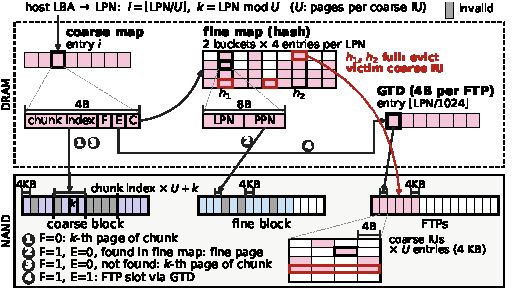
\includegraphics[width=\columnwidth]{figs/fig_design.pdf}
  \vspace{-6mm}
  \caption{DUET mapping structures.}
  \label{fig:design}
  \vspace{-2.5mm}
\end{figure}

\subsection{Two Mapping Granularities}
\textbf{Coarse map.} The logical space is divided into coarse IUs of $U$ pages
($4U$\,KB), so a logical page number (LPN) belongs to coarse IU $i=\lfloor \mathrm{LPN}/U \rfloor$ at
page offset $k=\mathrm{LPN} \bmod U$. Each coarse IU is stored as a \emph{chunk}
of $U$ physically consecutive, $U$-page-aligned pages in a \emph{coarse block},
and its 4\,B coarse entry holds the chunk index. Since a coarse entry covers $U$ pages and is as
large as a page-level entry, the coarse map takes $1/U$ of the DRAM of a page-level table.

\textbf{Fine map.} A write smaller than a coarse IU is written out of place as 4\,KB
\emph{fine pages} into separate \emph{fine blocks}. The fine map is a two-choice
bucketized hash table~\cite{balanced}. With two candidate
buckets, a bucket fills up much later than in an ordinary hash table with a
single candidate bucket~\cite{balanced}, so DUET evicts entries less often.
% ftlsim (results/coarse_gc/diag, end of run): mean fine pages per flagged IU 1.8 (fio) to 5.0 (YCSB-A) of U = 16,
% d <= 4 for 66-98% of IUs. Per-IU array 16 x 4 B = 64 B per IU vs 8 B x d in the table.
Each 8\,B entry holds an LPN and the
physical page number (PPN) of its fine page. Each LPN has two candidate buckets of four
entries each, and a new entry goes to the less loaded one. The table takes all of
the DRAM budget that the coarse map leaves.
% Implementation (92 GB, 1/8 budget): coarse map 5.6 MB, table 5.5 MB = fine pages of ~3% of logical pages.

The table is similar to cuckoo hashing~\cite{cuckoo} in that each entry has two
candidate buckets. Unlike cuckoo hashing, DUET never moves an existing entry to
its other bucket to make room, so an insert does not trigger a chain of moves.
When both candidate buckets are full, DUET instead writes the fine-map entries
of a victim coarse IU to a \emph{fine translation page} (FTP) in NAND and frees them
from the table (\emph{spill}, Section~\ref{sec:spill}). A table lookup therefore checks at most the eight
entries of the two candidate buckets, and an insert writes into a free entry of
one of them. A spilled entry has a fixed location in NAND, so one map-page
read returns it.

\textbf{Flag bits.} Each coarse entry also has three flag bits. The
\emph{has-fine-pages} (F) bit tells whether the coarse IU has fine pages, the
\emph{spilled} (S) bit tells whether their fine-map entries are in NAND, and the
\emph{clean} (C) bit tells whether the entries in the table are identical to their
copy in NAND (Section~\ref{sec:spill}).

\subsection{Host I/O Path}
\textbf{Read path.} A read first checks the coarse entry of coarse IU $i$. If F is set and S is clear, DUET
looks up the LPN in the fine map. If S is set, the global translation directory
(GTD)~\cite{dftl} locates the FTP of the
LPN, and DUET reads its slot. When the fine map or the slot points to a
fine page, DUET reads the fine page. Otherwise, including when F is clear, it
reads page $k$ of the chunk. A read thus reads at most three DRAM
locations, the coarse entry and the two candidate buckets. A 32\,B bucket lies
within one DRAM row, so each location costs one random DRAM
access~\cite{rixner}. Only a read of a spilled coarse IU adds one map-page read.

\begin{figure}[t]
  \centering
  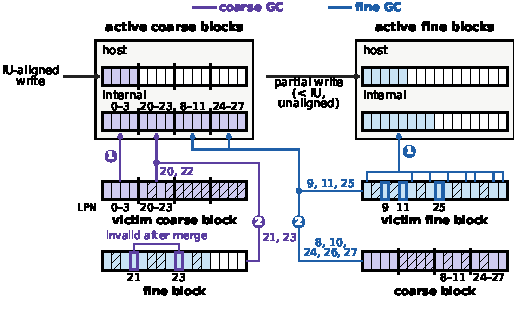
\includegraphics[width=\columnwidth]{figs/fig_write.pdf}
  \vspace{-8.5mm}
  \caption{DUET write and reclamation paths. Coarse GC (purple) and fine GC (blue) either (1) copy valid data or (2) merge it into new chunks.}
  \label{fig:write}
  \vspace{-2.5mm}
\end{figure}

\textbf{Write path.} Host writes go to two \emph{active blocks}, an active
coarse block for chunks and an active fine block for fine pages. A host write
is split at coarse-IU boundaries. Each IU-aligned write is written as a new chunk
in the active coarse block. The old chunk and all fine pages of the coarse IU
become invalid, and the corresponding fine-map entries are removed. If the coarse IU
already has fine pages, DUET instead writes the IU-aligned write as fine pages
while the fine blocks are below their cap (Section~\ref{sec:reclaim}).
% fine_full=1: keeps a hot coarse IU in the fine blocks instead of turning it back into a chunk on every full rewrite.

A \emph{partial write}, which is smaller than a coarse IU, is written as fine
pages into the active fine block. For each fine page, DUET inserts its LPN and
PPN into one of the two candidate buckets of the LPN, the less loaded one. The
page of the chunk with the same LPN becomes invalid. If the LPN already has a
fine page, DUET updates the PPN of its fine-map entry instead, and the old fine
page becomes invalid.

DUET keeps fine pages and chunks in different blocks. Fine pages hold recently
rewritten data and chunks hold colder data, and mixing data of different update
frequencies in one NAND block raises the GC cost~\cite{hotcold,dwf,multistream}.
As in other FTLs~\cite{sepbit}, DUET also separates host writes from internal
writes (GC and merges), so it keeps four active blocks (Figure~\ref{fig:write}).
When an active block is full, DUET takes a free block as the new active block.
% Final runs (results/final_vbm, q_vbm2.sh) use coarse_class=0 and uni_onefront=0, i.e. exactly four active blocks.
% Implementation also completes a nearly full partial write as a chunk when cheaper (eager RMW): 0.1-0.8% of host
% programs in the apps, 0 in traces / replays. Not described in the paper.

\subsection{Reclaiming Path}
\label{sec:reclaim}
DUET reclaims a block when the free blocks run low. Its written blocks
are divided into fine blocks, which hold fine pages, and coarse blocks,
which hold chunks.
DUET thus has two kinds of GC. \emph{Fine GC} reclaims a fine block, and
\emph{coarse GC} reclaims a coarse block. To find the valid data of a victim,
DUET keeps a valid bitmap with one bit per chunk slot of the coarse blocks and
one bit per page of the fine blocks.

\textbf{Coarse-or-fine victim selection.} DUET picks a victim with fewer valid pages to copy, whether it is a coarse
block or a fine block. The number of fine blocks, however, is limited by the OP
space. A fine page makes one page of a chunk invalid, but the chunk still takes
its place in a coarse block. The coarse blocks must therefore be able to cover
the whole logical capacity, and the fine blocks can only use the space beyond
it. When the fine blocks reach this cap, DUET thus reclaims a fine block.
Otherwise, it compares the coarse and fine blocks and runs GC on the side whose
block has fewer valid pages.
% Exact cap: OP blocks - GC reserve (T) - active blocks.
% Implementation: below the cap, the fewest-valid coarse and fine blocks are compared (gc_select_cost=1), and coarse GC
% then picks its actual victim by cost-benefit (not described in the paper).
% Ablation running (2026-11-06): greedy coarse victim on NVMeVirt, results/final_greedy (q_greedy.sh).
% ftlsim (results/coarse_gc pol:g): greedy raises WAF by 7.1% on average (up to 14.8% on TPC-C).

% Dropped (victim policy left implicit, "fewer valid pages to copy" in Victim selection): coarse GC picks its victim by
% cost-benefit [lfs], weighing block age so a recently written block gathers more invalid pages. Fine GC is greedy.
\textbf{Coarse GC.} Coarse GC handles each valid chunk of the victim in
one of two ways (purple lines in Figure~\ref{fig:write}). A chunk whose coarse
IU has no fine pages (LPN 0--3) is copied unchanged to a new chunk (\cgc{1}). A
chunk whose coarse IU has fine pages (LPN 20--23) is only partly valid, so DUET
merges it (\cgc{2}). DUET looks up the LPNs of the coarse IU in the fine map.
An LPN found there has a fine page (LPN 21 and 23), and an LPN not found there
is still valid in the chunk (LPN 20 and 22). DUET reads these pages and writes
them as one merged chunk. The fine pages then become invalid, their fine-map
entries are removed, and the F bit of the coarse IU is cleared.

\textbf{Fine GC.} Fine GC handles each coarse IU with valid fine pages in the victim in one of two ways
(blue lines in Figure~\ref{fig:write}). DUET either copies the fine pages to
another fine block (\fgc{1}) or merges the coarse IU with its chunk (\fgc{2}).
In Figure~\ref{fig:write}, LPN 9 and 11 are merged with the chunk of LPN 8--11,
and LPN 25 with the chunk of LPN 24--27. Let $d$ be the number of fine pages
of the coarse IU in all fine blocks, not only in the victim. A merge reads the
chunk and these $d$ fine pages and writes one new chunk. All $d$ fine pages then
become invalid, and their fine-map entries are removed.

\textbf{Copy-or-merge decision.} DUET chooses one of the two ways by a cost-benefit model. The cost is the
number of pages written, and the benefit is the number of pages freed in the
fine blocks. Let $P$ be the number of pages per block, $v$ the number of valid
pages in the victim, and $U$ the number of pages in a coarse IU. For the same
victim, copying costs $v$ page writes and frees $P - v$ pages. A merge of a
coarse IU with $d$ fine pages instead costs $U$ page writes, one coarse IU, and
frees its $d$ fine pages. The cost-benefit value, that is, the number of pages
freed in the fine blocks per page written, is thus $(P-v)/v$ for copying
(\fgc{1}) and $d/U$ for a merge (\fgc{2}). DUET copies the fine pages when
$(P-v)/v \ge d/U$, and otherwise merges the coarse IU. DUET makes this decision for
every coarse IU that has valid fine pages in the victim fine block.
% Implementation also keeps hot fine pages (cost_cold, rec_block=1): no merge if a fine page of the IU sits in a host
% fine block newer than the victim. Not described in the paper.

\textbf{Fine-area size.} The number of fine blocks and the number of fine-map entries
change at runtime with these two decisions. When coarse-or-fine victim selection
often picks a coarse block, fine pages accumulate in the fine blocks, and the number
of fine blocks grows up to the OP limit. When it often picks a fine block, the number
of fine blocks shrinks. The copy-or-merge decision then sets the number of fine-map
entries. Copying keeps the fine pages and their fine-map entries, so the fine map
grows as new small writes arrive, whereas a merge moves the fine pages into a chunk
and frees their fine-map entries, so the fine map shrinks. The size of the fine map
thus adapts to the workload (Section~\ref{sec:eval}).

\subsection{Fine-Map Spill and Load}
\label{sec:spill}
Under a fixed DRAM budget, the table cannot index every fine page that the fine
blocks can hold. For example, a budget of 128\,MB per TB of capacity, 1/8 of
the page-level table, holds the whole map of an SSD with uniform 32\,KB coarse IUs. If
DUET uses 64\,KB chunks under this budget, the coarse map takes 64\,MB per TB.
Since each fine-map entry takes 8\,B, the remaining 64\,MB holds about 8M
entries, which map 32\,GB of fine pages. If the fine blocks use all of
the 7\% OP space, however, they can hold 70\,GB of fine pages per TB. The table thus has no room for more
than half of their fine-map entries. The DRAM capacity is fixed when the SSD hardware is designed.
Unlike the FTL, which can be updated with the firmware, it cannot be changed easily.
% Illustration: 7% of 1 TB = 70 GB vs 32 GB in the table -> 54% do not fit. (Device: fine cap 18 blocks after GC reserve and active blocks, 1 - 334,736 / 557,568 = 40%.) Per TB: table 334,736 / L 10,798,160 = 3.10% of logical pages = 31.7 GB, fine cap 557,568 / L = 5.16% = 52.9 GB. FAST under the same budget (old text): rwcap=14 of nlog=23, 8 spare blocks unused.
% Numbers: apps device P=30976, fine cap 18 blocks = 557,568 pages, cuckoo2 table 334,736 entries (spill=2, GTD charged).
% FAST (results/final_rp apps dmesg): NB=373 NLB=348 T=2 -> nlog=23, cache_bytes=B12 -> rwcap=14 (SW + 14 RW = 15 log blocks).

Another challenge is hash collisions within the fine map. An insert can find
both of its candidate buckets full even when other buckets still have free slots.
Hashing schemes that place a colliding entry in another
bucket~\cite{cuckoo,onemove,hopscotch,robinhood} make a lookup probe more buckets or an
insert move existing entries, so they need more DRAM accesses. On the other hand,
merging the coarse IU whose entries are pushed out of the full buckets into the coarse map
causes extra NAND writes.

DUET instead keeps the fine-map entries of some coarse IUs in FTPs in NAND, so the
fine blocks can use all of the OP space without more DRAM.
The fine-map entries of a coarse IU move to its FTP when the table fills
(\emph{spill}) and back to the table when the coarse IU is accessed again
(\emph{load}), and no data moves in either direction. In theory, the spilled entries map
at most 7\% of the data, the size of the OP space, because most data are mapped by the
coarse map, which is always in DRAM.
% Bound: spilled <= fine pages <= OP (7%). Spill can start before the table is full (bucket pairs fill unevenly), so
% 70 - 32 GB is not a bound. Measured: YCSB-A max spilled 312,824 / L 10,798,160 = 2.9% (results/final_stats).

\textbf{Spill.} As shown in Figure~\ref{fig:design}, the fine-map entry of each LPN has a
fixed 4\,B slot in an FTP,
which holds the entries of 1024 consecutive LPNs. As in DFTL, the GTD locates each
FTP with one 4\,B entry, charged to the same DRAM budget. When an insert finds both
candidate buckets full, DUET picks a victim among the coarse IUs that have an entry in
the two buckets. It writes all entries of the victim to its FTP, sets its S bit, and
frees its table entries. The other coarse IUs of the same FTP are spilled with the
same program.

\textbf{Load.} An access to a spilled coarse IU reads its FTP and loads only the
entries of that coarse IU into the table. The other
coarse IUs of the FTP stay spilled. A write loads the entries and then updates them.
A read reads the FTP before the data, loads the entries, and sets the C bit of the
coarse IU. The coarse IU stays clean until one of its entries changes.

\textbf{What to spill.} DUET picks a clean coarse IU first to reduce FTP writes to NAND.
A clean coarse IU is simply dropped from the table and marked spilled because its FTP
copy is still valid. If there is no clean coarse IU, DUET picks the coarse IU with the
most fine pages, so one FTP program frees the most table slots.
% Code: prop_ct_best(pc = spill_rp_clean) prefers clean IUs among the bucket pair, then most fragments, then older.

\textbf{GC.} When GC moves fine pages of spilled coarse IUs, it reads and programs
each FTP at most once per victim block. A merge of a spilled coarse IU reads its
entries from the FTP and then clears its F and S bits.
% Dropped detail (2026-11-06): one recently used FTP is kept in controller SRAM. A coarse IU becomes dirty when one of its
% fine pages changes (write, merge, GC copy).

% Overhead subsection removed (2026-11-07): DRAM parts are in Sections A and D, the three DRAM accesses in the read path.
% Left for the eval setup: mapping reads and programs (spilled coarse IUs only) are counted in all WA and latency results.
